
%place your content here, feel free to create subcontent files

\begin{block}{\blocktitle{Abstract}}
\justifying
We propose minimum regret search (MRS), a \emph{novel acquisition function} for Bayesian
optimization. MRS bears similarities with information-theoretic approaches
such as entropy search (ES). However, while ES aims in each query at maximizing the
information gain with respect to the global maximum, MRS aims at \emph{minimizing the
expected simple regret} of its ultimate recommendation for the optimum. While empirically ES and MRS perform similar in most of the
cases, MRS produces fewer outliers with high simple regret than ES. We provide empirical
results for a synthetic single-task optimization problem.
\end{block}

\begin{block}{\blocktitle{Background}}
\textbf{Bayesian optimization} \cite{shahriari_taking_2016}:
\begin{itemize}
\item black-box optimization problems $\mathbf{x} = \arg\max_{\mathbf{x} \in \mathcal{X}} f(x)$ of some function $f: \mathcal{X} \to \mathbb{R}$ on some bounded set $\mathcal{X} \subset \mathbb{R}^D$.
\item maintains a \emph{probabilistic model} $p(f)$ for $f(\mathbf{x})$, typically a Gaussian process (GP)
\item decides on a query point $\mathbf{x}_{n+1}$ where $f$ will be evaluated next based on GP posterior after first $n$ observations $\mathcal{D}_n=\{(\mathbf{x}_i, y_i)\}_{i=1}^n$ and an \emph{acquisition function}
\item recommends $\mathbf{\tilde x}_N$ as optimum after $N$ queries (optimum of GP or best query point)
\item objective: minimize \emph{simple regret} 
$R_f(\mathbf{\tilde  x}_N) = f(\mathbf{x}^\star) - f(\mathbf{\tilde  x}_N) = \max_{\mathbf{x}} f(\mathbf{x}) - f(\mathbf{\tilde x}_N)$
\end{itemize}

Acquisition functions decide where to query next:
\begin{itemize}
\item Upper-Confidence Bound (UCB): $a_{UCB}(\mathbf{x};
\mathcal{D}_n) = \mu_{n}(\mathbf{x}) + \kappa_n \sigma_{n}(\mathbf{x})$
\item Probability of Improvement (PI): $a_{PI}(\mathbf{x}; \mathcal{D}_n) := \mathbb{P}[f(\mathbf{x}) > \tau]$
\item Expected Improvement (EI): $a_{EI}(\mathbf{x}; \mathcal{D}_n) := \mathbb{E}[(f(x) - \tau)\mathbb{I}(f(x) > \tau)]$
\item Entropy Search (ES) \cite{hennig_entropy_2012}: $a_{ES}(\mathbf{x}, \mathcal{D}_n)
  = H(\mathbf{x}^\star \vert \mathcal{D}_n) - \mathbb{E}_{y \vert \mathbf{x}, \mathcal{D}_n}
	[H(\mathbf{x}^\star \vert \mathcal{D}_n \cup \{(\mathbf{x}, y)\})]$,
	where $H(\mathbf{x}^\star \vert \mathcal{D}_n)$ denotes the differential entropy
of the posterior distribution $p^\star(x \vert \mathcal{D}_n)$ of the unknown optimizer $\mathbf{x}^\star = \arg\max_{\mathbf{x} \in \mathcal{X}} f(\mathbf{x})$.
\end{itemize}

\end{block}

\begin{block}{\blocktitle{Minimum Regret Search (MRS)}}

Acquisition function based directly on external objective of minimizing simple regret
\begin{itemize}
 \item Expected simple regret: $\text{ER}(p)(\mathbf{x}) = \mathbb{E}_{p(f)}[R_f(\mathbf{x})]
= \mathbb{E}_{p(f)}[\max_{\mathbf{x}} f(\mathbf{x}) - f(\mathbf{
x})]$
 \item For fixed GP $p(f)$, $\arg\min_\mathbf{x} \text{ER}(p)(\mathbf{x})$ corresponds to the maximizer of the GP mean
 \item MRS aims at selecting query points s.t.\  ER is minimized also with respect to resulting $p(f)$
 \item Myopic choice: select next query point s.t.\ minimum ER is reduced the most (in expectation)
 \item $a_{\text{MRS}^{\text{point}}}(\mathbf{x}^q)
	= \min_{\mathbf{\tilde x}}\text{ER}(p_n)(\mathbf{\tilde x})
	 - \mathbb{E}_{y \vert p_n(f), \mathbf{x}^q}[\min_{\mathbf{\tilde x}}  \text{ER}(p^{[\mathbf{x}^q, y]}_n)(\mathbf{\tilde x})]$
 \item Additionally also accounting for uncertainty in minimizer $\mathbf{\tilde x}$ of $\text{ER}$ yields MRS
 \item $a_{\text{MRS}}(\mathbf{x}^q)
    = \mathbb{E}_{\mathbf{\tilde x} \sim p^\star_{\mathcal{D}_n}}[\text{ER}(p_n)(\mathbf{\tilde x})] 
	   - \mathbb{E}_{y \vert p_n(f), \mathbf{x}^q}[
		  \mathbb{E}_{\mathbf{\tilde x} \sim p^\star_{\mathcal{D}_n \cup \{(\mathbf{x}^q, y)\}}}[
			 \text{ER}(p^{[\mathbf{x}^q, y]}_n)(\mathbf{\tilde x})]]$
\end{itemize}

Approximate $a_{\text{MRS}}$ based on sampling:
\begin{itemize}
 \item approximate $\mathbb{E}_{p(f)}$ by taking $n_f=1000$ Monte Carlo samples from $p(f)$
 \item approximate $\mathbb{E}_{y \vert p(f), \mathbf{x}^q}$  by taking
$n_y=51$ Monte Carlo samples from $p(f)$'s predictive distribution at
$\mathbf{x}_q$
 \item discretize $p^\star$ to a finite set of $n_r=25$ representer points (Thompson
sampling from $p(f)$ on candidate points)
 \item estimating $p^\star_{\mathcal{D}_n}$ on representer points by reusing the samples used 
for approximating $\mathbb{E}_{p(f)}$ (incurs a small bias)
\item Common random numbers in estimation of
$\text{ER}(p)(\mathbf{x})$ for different $p(f)$ reduces variance
\end{itemize}
\end{block}

\begin{block}{\blocktitle{Illustration}}
\vspace*{1cm}

\begin{figure}
\centering
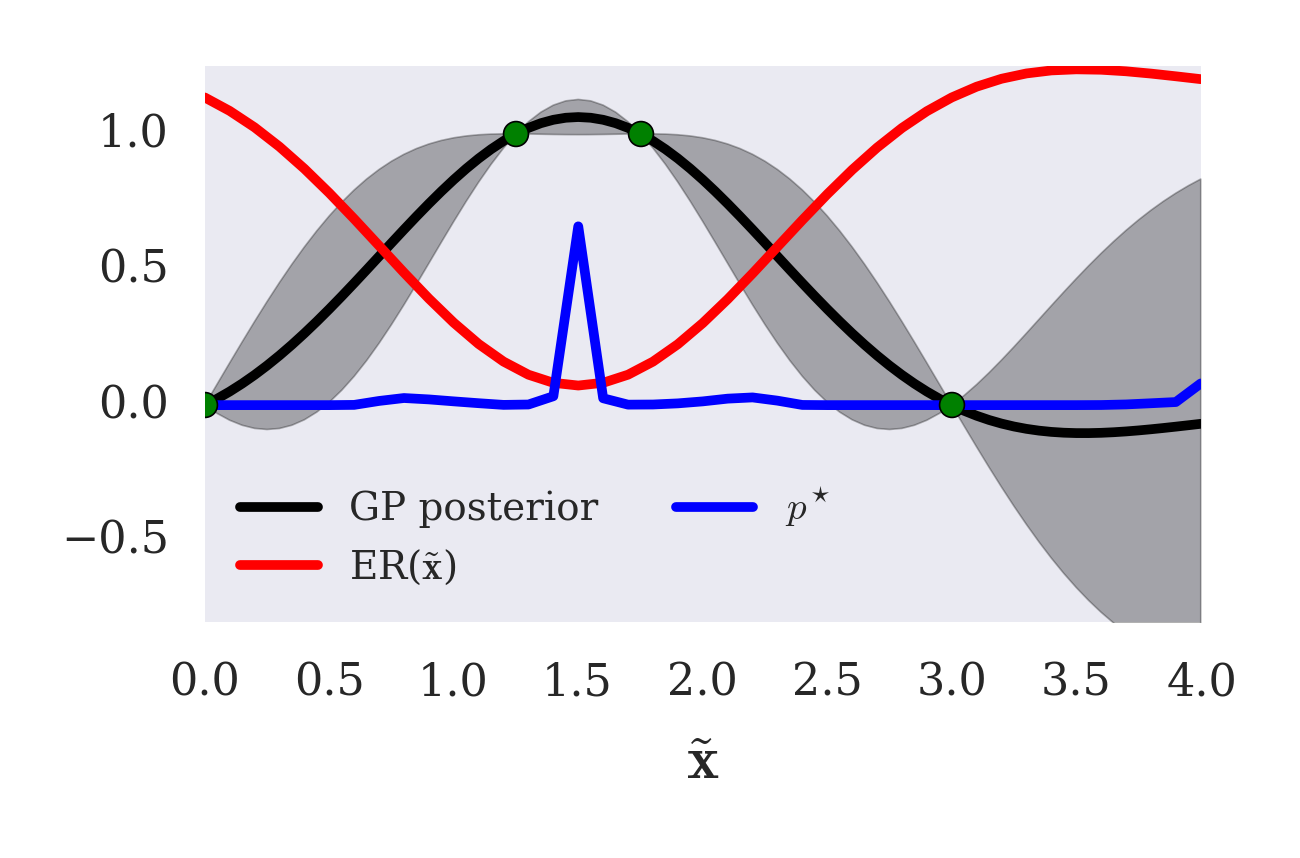
\includegraphics[width=0.48\columnwidth]{../pics/regret_illustration_2}
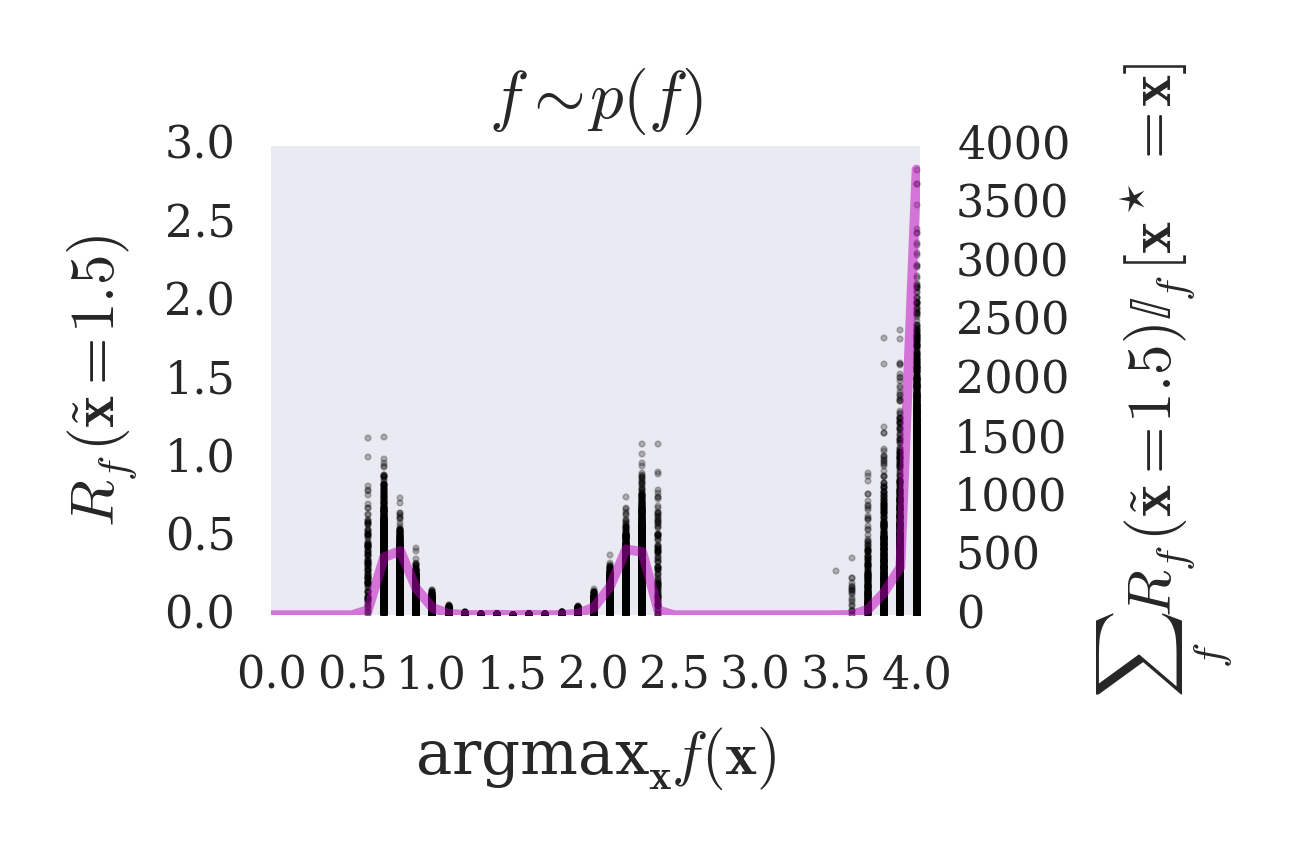
\includegraphics[width=0.48\columnwidth]{../pics/regret_scatter}
\caption{(Left) GP posterior, probability of maximum $p^\star$, and expected regret ER. (Right) Scatter plot of position of optimum and regret of $\mathbf{\tilde x} = 1.5$ versus optimum in sample functions.}
\label{fig:MRS_illustration}
\end{figure}

\begin{figure}
\centering
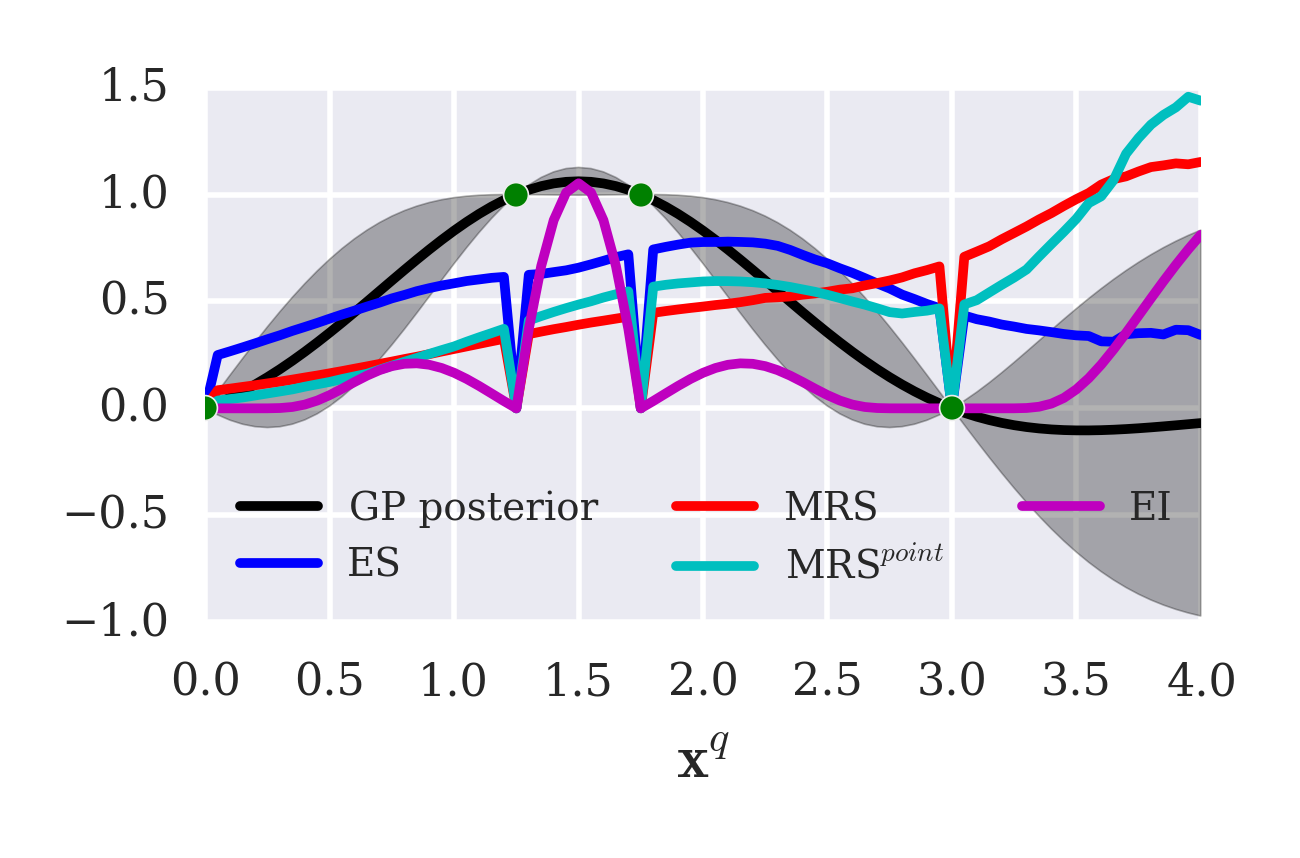
\includegraphics[width=0.48\columnwidth]{../pics/acq_comparison}
\caption{GP posterior and different acquisition function. Absolute values have been normalized such that the mean value of acquisition function is $0.5$.}
\label{fig:MRS_illustration}
\end{figure}
\end{block}
